This first approach is most similar to Sequential Deep Belief Networks in that it learns a transition operator between hidden latent states \(H\). This model uses the power of GSN's to learn hidden representations that vastly reduce the complexity of the input data space, making transitions between data manifolds at higher layers of representation much easier. Therefore, the transition step of learning \(H \rightarrow H\) over time should be less complicated (only needing a single linear regression step). This model uses both artificial time-sequencing (for the GSN training to have backpropagation through time to learn the data manifolds), as well as real time-sequencing (for the regression step). Alternating between training the GSN parameters on the generative input sequence through Gibbs sampling and learning the hidden state transition operator on the real sequence of inputs allows the model to tune parameters quickly in an expectation-maximization style of training.



\section{Recurrent nature of deep GSNs}

While GSNs are inherently recurrent and depend on the previous latent and visible states to determine the current hidden state, \(H_{t} \sim P_{\Theta_1}(H|H_{t-1},X_{t-1})\), this time series \(t\) is artificial and generated through the GSN sampling process. Using this sampling process, GSNs actively mix between modes that are close together in the input space, not the sequential space. For example, a GSN trained on MNIST data will learn to mix well between the modes of digits that look similar in the pixel space - sampling from the digit "0" transitions to an "8", etc.

\begin{figure}[h!]
  \centering
    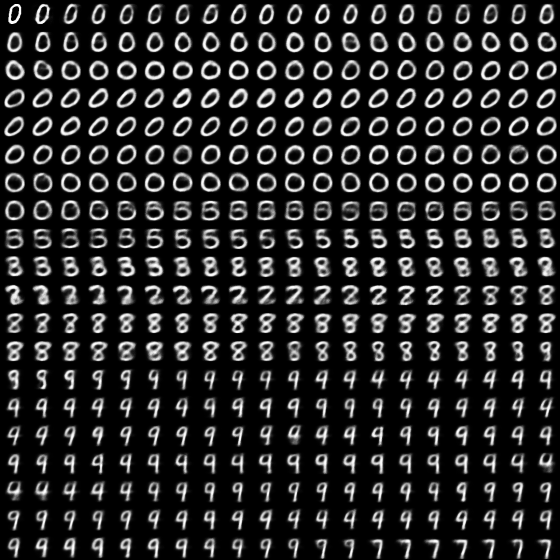
\includegraphics[width=0.8\textwidth]{gsn_samples}
\caption{Samples from GSN after 300 training epochs. Good mixing between major modes in the input space.}
\end{figure}



\section{Algorithm}



\section{Experimental results}

